\newpage
\pagenumbering{arabic}

\hypertarget{einleitung-motivation-fragestellung}{%
\section{Motivation und Fragestellung}\label{einleitung-motivation-fragestellung}}

Ein langfristiges Projekt ist das Bauen einer autarken Wetterstation
basierend auf dem Raspberry~Pi\footnote{raspberrypi.org}. Dies ist ein
linuxbasierter Einplatinencomputer (System-On-A-Chip, SoC). Es werden
die Temperatur, Luftfeuchtigkeit und Luftdruck von Sensoren gemessen.
Langfristig soll die Wetterstation nicht nur aktuelle Wetterdaten
aufzeichnen und grafisch aufbereiten, sondern das Wetter auch
vorhersagen. Da sich verschiedene Wolkentypen bei unterschiedlichen
Witterungsverhältnissen bilden, kam die Idee auf, die aktuelle
Wolkenlage als Parameter der Wettervorhersage zu nutzen. Insbesondere
die Veränderungen der Wolkenlage lässt eindeutige Rückschlüsse über den
Verlauf des Wetters zu.

Die Rechenleistung und der verfügbare Speicher des Raspberry~Pi ist
gering, sodass es sinnvoll ist, die notwendigen Rechnungen und den
Umfang aufgenommener Daten zu beschränken. Aus diesem Grund soll die
autarke Wetterstation nur den aktuellen Wolkentyp für die Vorhersage
speichern.

Die Wetterstation ist mit einer Kamera bestückt, die regelmäßig
Wetterdaten und Himmelfotos aufnimmt. Diese Fotos sollen klassifiziert
werden, sodass die Datenspeicherung aus einer Klassenrepräsentation,
statt aus einem Foto besteht.

Ein maschinelles Lernverfahren soll genutzt werden, um die Himmelfotos
direkt auf dem Raspberry~Pi zu klassifizieren. Die Wahl fällt auf ein
Neuronales Netz. Neuronal Netze bestehen aus mehreren Schichten, die
verschiedene Matrixmultiplikationen verwenden, um zum einen Dimensionen
zu reduzieren und zum anderen Eingangsparameter im Bezug auf die zugehörige Klasse
zu gewichten. Ein großer Vorteil gegenüber anderen maschinellen
Lernverfahren ist, dass das Modell unabhängig von den Trainingsdaten
verwendet werden kann (vergleiche kNN, hier muss der gesamte
Trainingsdatensatz gespeichert werden), was für die Wettervorhersage
sehr sinnvoll ist, da der Speicherplatz begrenzt ist (s.~o.). Außerdem
besteht so die Möglichkeit, mehrere Wetterstationen zu kombinieren und
für die Klassifikation muss nur das Modell weitergegeben werden. Die
Matrixmultiplikationen sind der Grund dafür, dass die Auswertungszeit
auch mit geringer Rechenleistung kurz bleibt. Ein Neuronales Netz wird
mit sogenannten \texttt{Convolutional} Schichten die Formen der
Wolkenklassen lernen und zusammen mit den Information der drei
Farbkanäle (rot, grün, blau) in \texttt{Dense} Schichten gewichten, um
eine Klassifikation zu ermöglichen.

Eine Alternativmethode zum Neuronalen Netz ist der Random Forest. Auch
hier kann das Modell zum Auswerten ohne die Trainingsdaten weitergegeben
werden und ist somit gut geeignet für kleine Systeme wie den Raspberry~Pi.
Der Random Forest hat weniger Kapazitäten als das Neuronale Netz, da
er nur die Information der Farbkanäle zum Trainieren bekommt. Der Random
Forest ist ein beliebter Algorithmus für maschinelles Lernen, da er mit wenig
Optimierung brauchbare Ergebnisse liefert und seine Trainingszeit sehr
gering ist. Ein Random Forest besteht aus einem Ensemble von mehreren
binären Entscheidungsbäumen.

\hypertarget{auswahl-und-beschreibung-des-datensatzes}{%
\section{Auswahl und Beschreibung des
Datensatzes}\label{auswahl-und-beschreibung-des-datensatzes}}

Der Raspberry~Pi nimmt regelmäßig Fotos auf. Diese werden von uns in 11
Klassen eingeteilt und gelabelt.
Die Verteilung der Klassen ist in Abbildung~\ref{fig:verteilung} dargestellt.
Dazu haben wir einen
\texttt{Telegram-Bot}\footnote{@weatherpi\_bot} erstellt, der uns und
anderen freiwilligen Helfern Fotos geschickt hat, die dann zu labeln
sind.

\begin{figure}
\centering
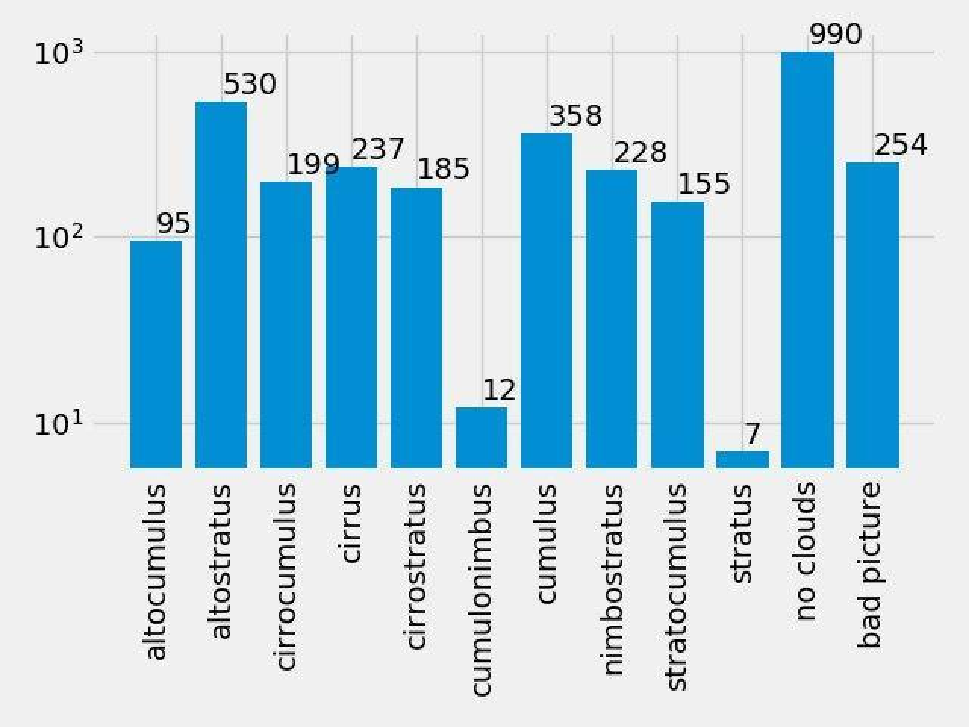
\includegraphics[width=0.8\textwidth]{content/histogramm_samples.pdf}
\caption{Verteilung der Klassen.}%
\label{fig:verteilung}
\end{figure}

Besonders hervorzuheben sind `Bad Pictures', da auf diesen zum einen
gar kein Himmel zu sehen ist, da die Kamera in die falsche Richtung
gezeigt hat, zum anderen unbekannte Fehler während der
Aufnahme auftraten.
Siehe für Beispiele Abbildung~\ref{fig:fehler}.

\begin{figure}
  \centering
  \begin{subfigure}[t]{0.48\textwidth}
    \centering
    
\includegraphics[width=\textwidth]{pictures/bad_3.pdf}
    \caption{Unbekannter Fehler während der Aufnahme.}%
    \label{subfig:fehler1}
  \end{subfigure}

  \begin{subfigure}[t]{0.48\textwidth}
    \centering
    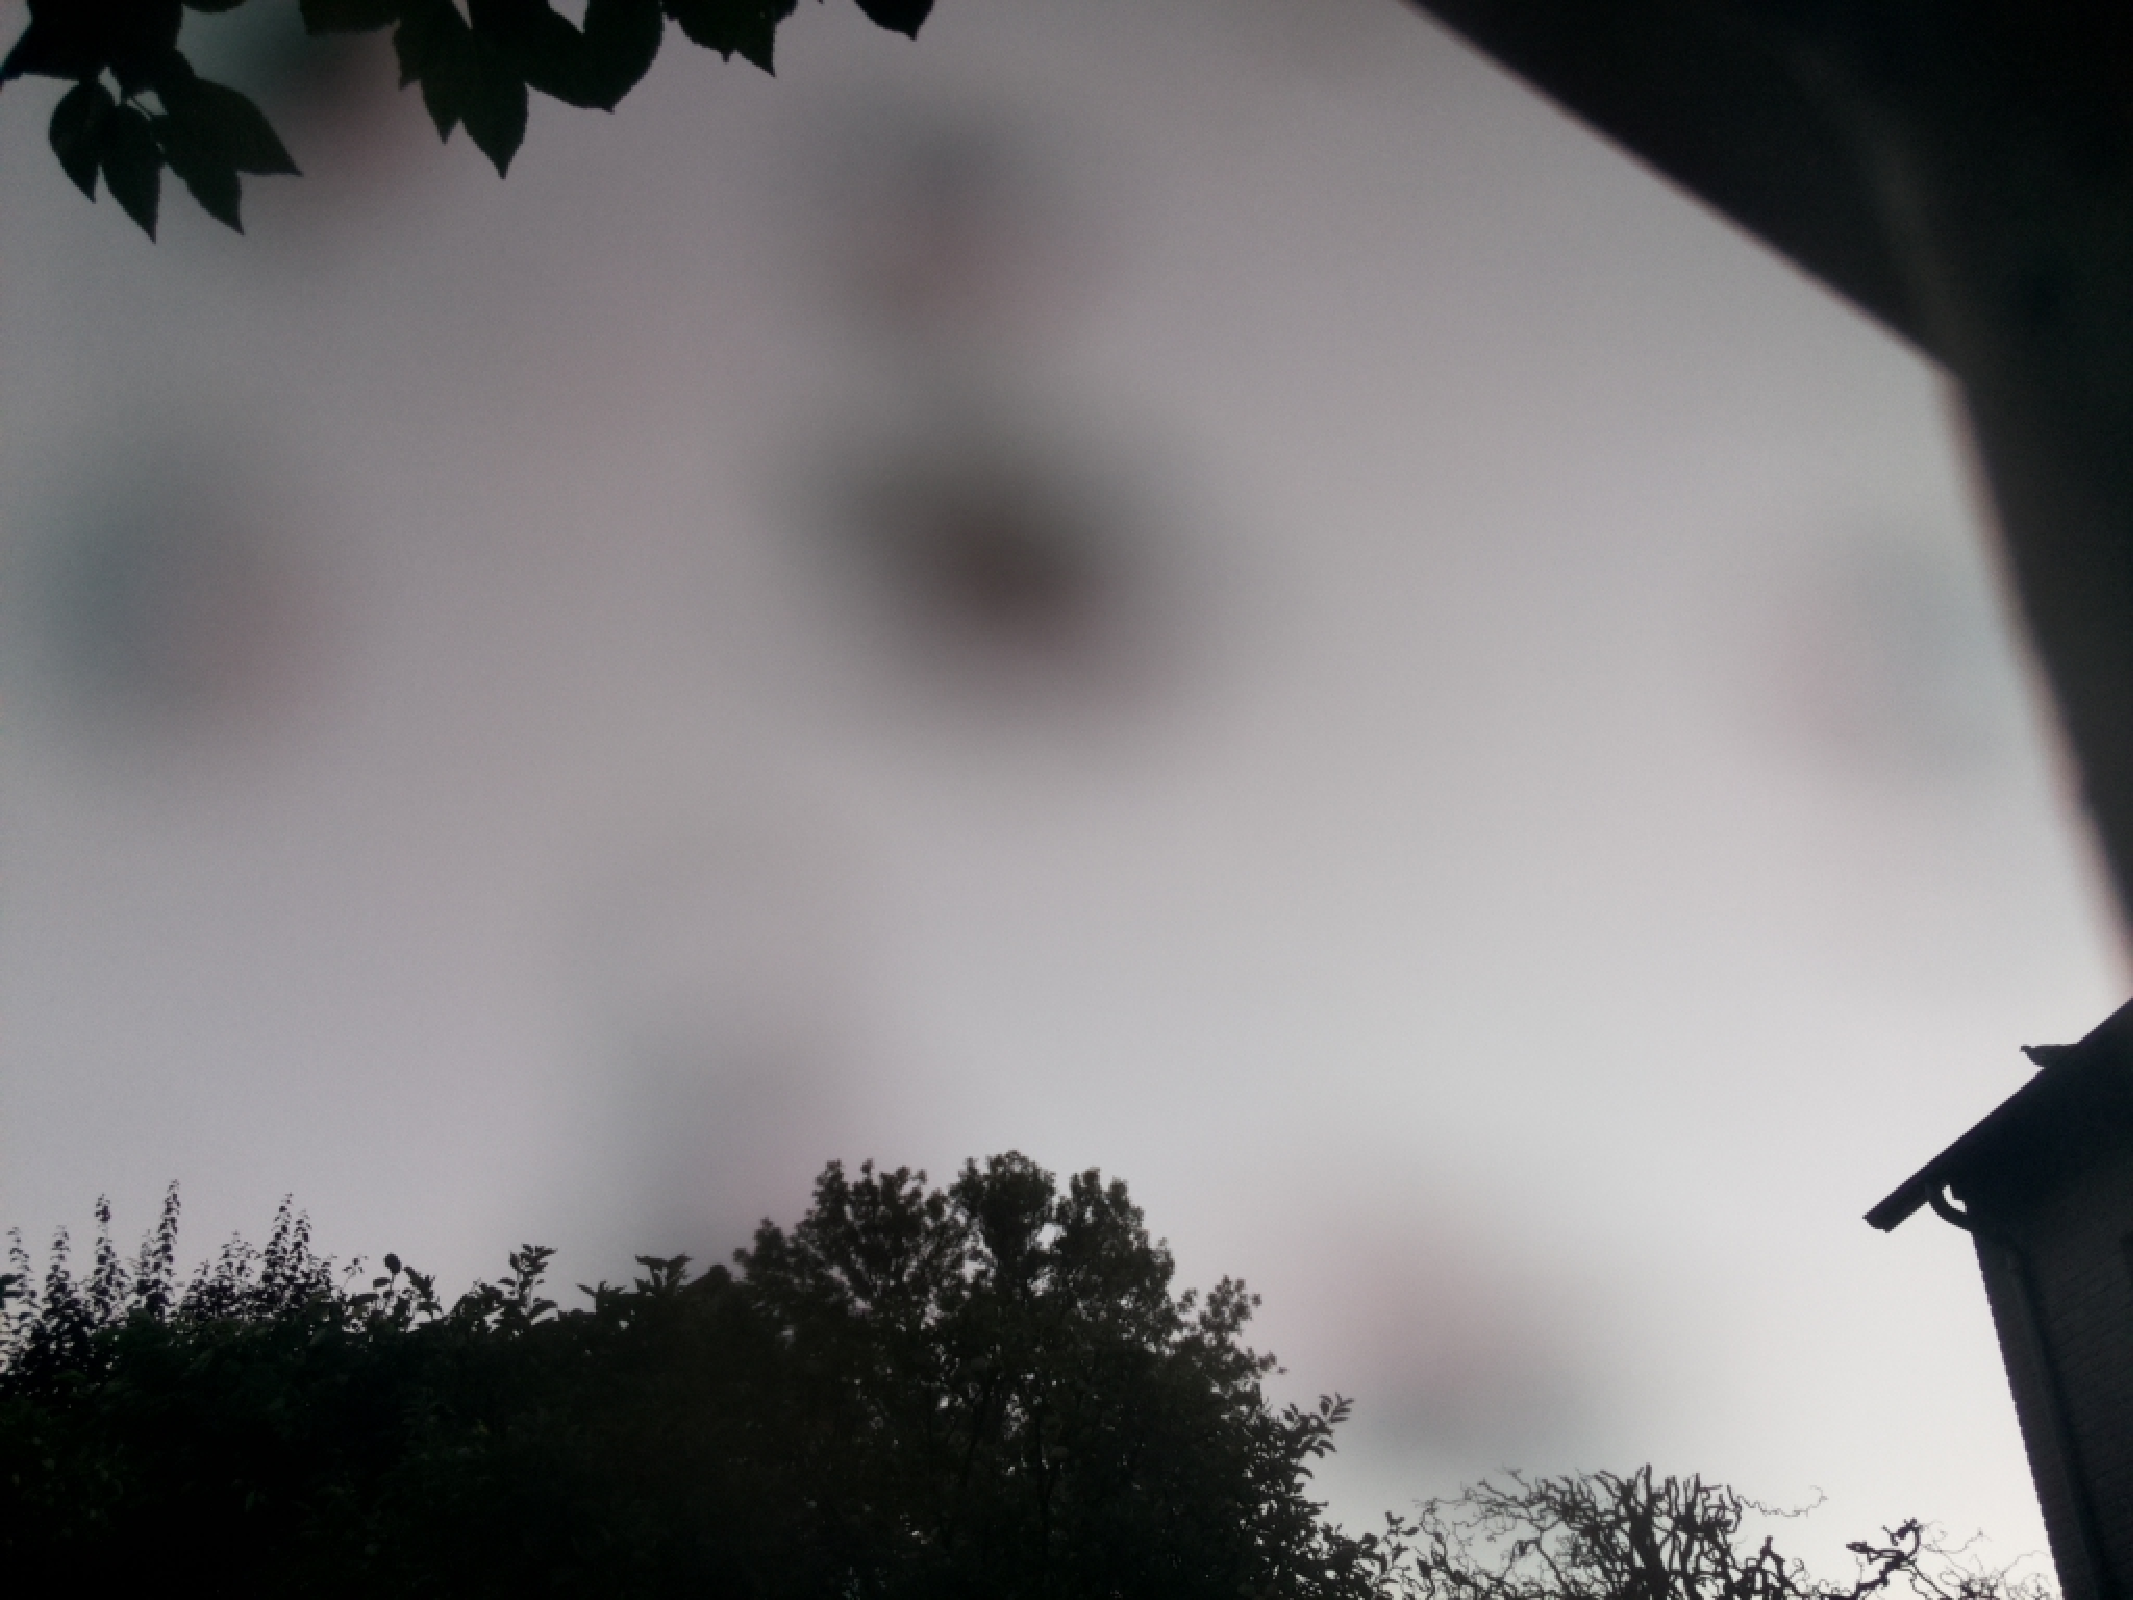
\includegraphics[width=\textwidth]{pictures/bad_rain.pdf}
    \caption{Regentropfen auf der Kameralinse erschweren das Labeln.}%%
    \label{fig:rain}
  \end{subfigure}
  \begin{subfigure}[t]{0.48\textwidth}
    \centering
    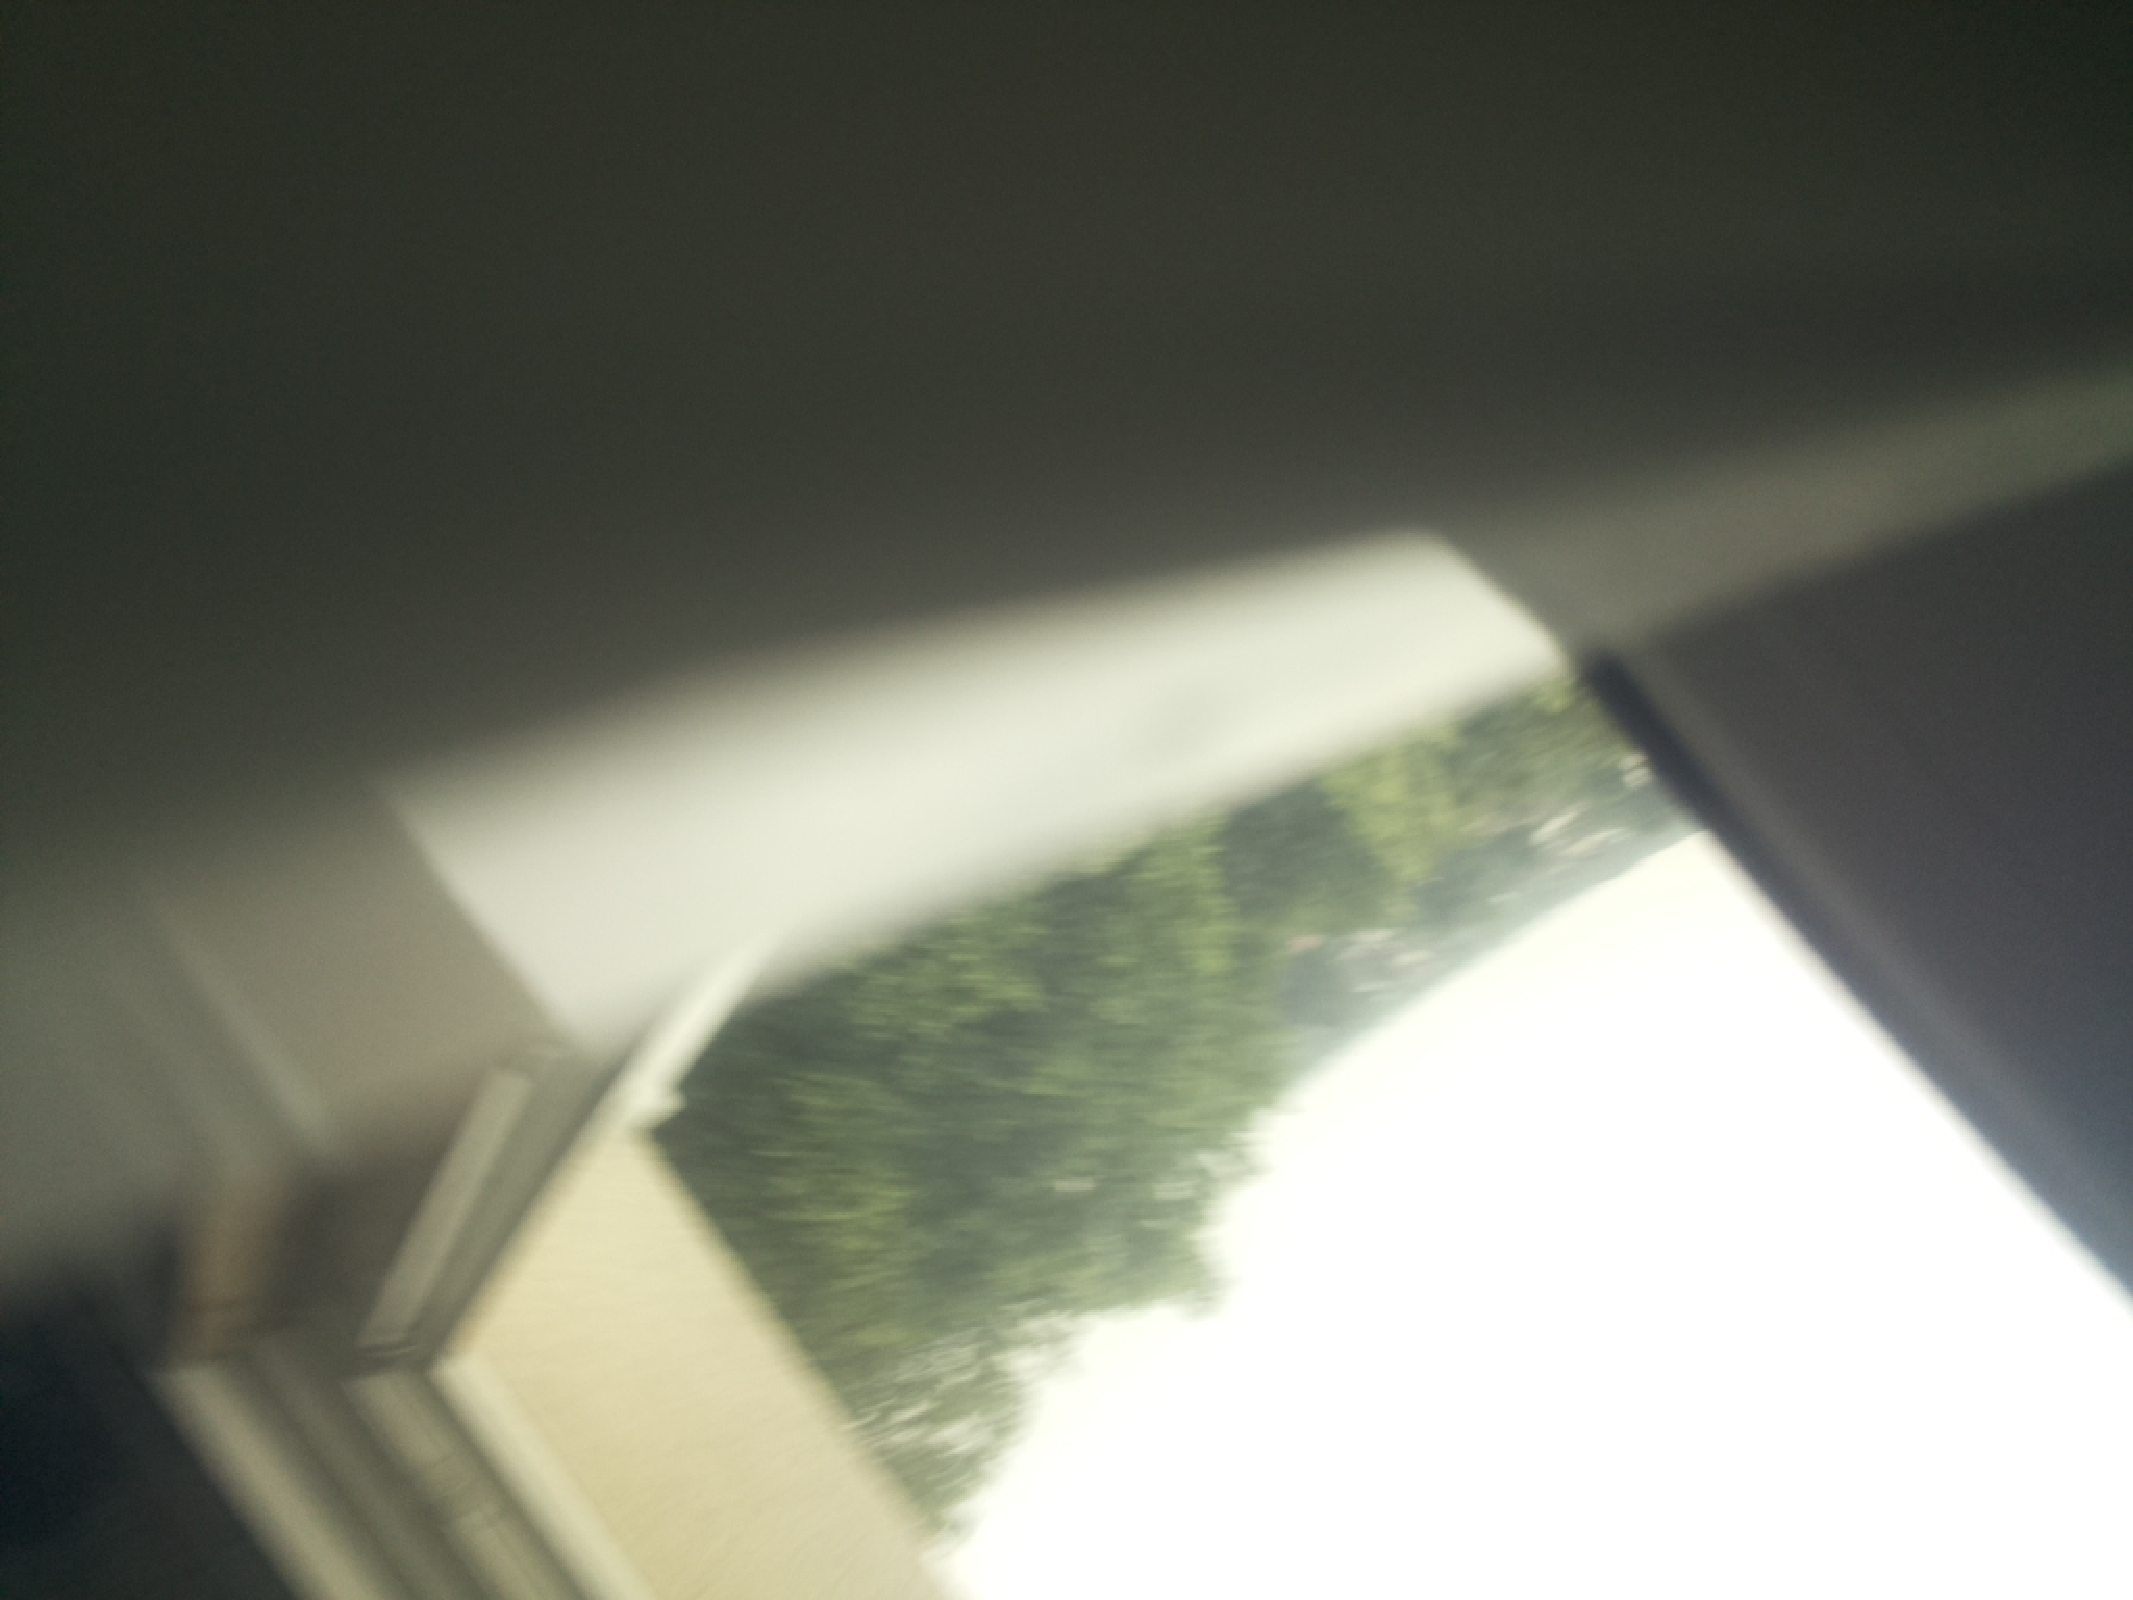
\includegraphics[width=\textwidth]{pictures/bad_2.pdf}
    \caption{Beispiel für \enquote{falsche Richtung}.}%
    \label{fig:wrong_direction}
  \end{subfigure}
  \caption{Beispiele für `Bad Pictures'.}%
  \label{fig:fehler}
\end{figure}

Auf weiteren `Bad Pictures' sind zu
viele Regentropfen auf der Kameralinse, sodass eine vernünftige
Klassifikation von unserer Seite nicht zuverlässig wäre,
was einen unreinen Datensatz zur Folge hätte.
Weiterhin nimmt die Wetterstation auch nachts Fotos auf, welche aufgrund
des schlechten Lichtsensors in der Kamera nicht gut aufgelöst werden
können uns somit großflächig zu dunkel sind, um Wolken zu erkennen.

Fotos bei Nacht und `Bad Pictures' werden nicht mit abgegeben, um den
benötigten Speicherplatz für den Datensatz nicht unnötig zu vergrößern.
Die beiden Klassen werden auch nicht in das Training der Algorithmen
aufgenommen, da die selbstgestellte Aufgabe ist, fotografierte Wolken in
Wolkenklassen einzuteilen, nicht zu entscheiden, ob es ein gutes
(persönliche/menschliche Wertung) Foto ist. Auf langfristige Sicht
sollte der Anteil von `Bad Pictures' statistisch gering sein.

Der Datensatz besteht ohne `Bad Pictures' und Fotos bei Nacht aus 3250
Fotos mit 1024$\times$768 Pixeln mit je 3 Farbkanälen und belegt unkomprimiert
1,5 GB Speicherplatz. Er ist aufgeteilt in 11 Wolkenklassen, von denen 2
aus weniger als 12 Fotos bestehen.

Der Datensatz wird freigegeben unter der MIT-Lizenz.

\hypertarget{motivation-und-darstellung-des-luxf6sungsansatzes}{%
\section{Motivation und Darstellung des
Lösungsansatzes}\label{motivation-und-darstellung-des-luxf6sungsansatzes}}

Im Folgenden wird erklärt, wie die aufgenommenen Fotos vorverarbeitet
werden und wie sich die Architekturen und das Training der maschinellen
Lernverfahren auf die gewählten Leistungsmerkmale auswirken.

\hypertarget{vorverarbeitung}{%
\subsection{Vorverarbeitung}\label{vorverarbeitung}}

Zuerst werden Fotos bei Nacht aus dem Datensatz entfernt. Die erste Idee
war, die Fotos anhand der Aufnahmezeit zu filtern. Dies wurde schnell
verworfen, da bewusst war, dass bei einer langfristigen Nutzung der
Wetterstation die Zeiten der Sonnenauf- und -untergänge variieren. Die
Fotos werden stattdessen bei einer mittleren Pixelhelligkeit unter 70
verworfen. Dies hat den Vorteil, dass keine Rücksicht auf den Standort
und die Systemzeiteinstellung verschiedener Wetterstationen Rücksicht
genommen werden muss.

Die Aufnahme ist so programmiert, dass die Fotos noch vor dem
Abspeichern den Helligkeitsfilter durchlaufen, sodass dunkle Fotos nicht
gespeichert werden.

Anschließend werden Schnitte auf den Farbkanälen der einzelnen Fotos
angewendet. Dies geschieht aus zwei Gründen, die in der dargestellten
Reihenfolge während der Arbeit aufkamen:

\begin{itemize}
\item
  Entfernung von fotografierten Objekten, die nicht zum Himmel gehören.
  Hierzu zählen insbesondere Bäume und Hauswände, die sich im Sichtfeld
  der Kamera befinden. Diese Objekte sollen mit einem allgemein
  anwendbaren Algorithmus, anstelle eines harten Schnittes auf
  entsprechenden Bildregionen, entfernt werden, damit verschiedene
  Wetterstationen denselben Code verwenden können.
\item
  Entfernung von Farbwerten wie grün und rot, die im Farbraum von den
  dominanten Himmelfarben blau, weiß und grau weit entfernt sind, damit
  die Parameter des Random Forest die Himmelfarben und nicht
  Umgebungsfarben sind.
\end{itemize}

Es wird hierzu ein Schnitt der Form einer im Farbraum rotierten Parabel
mit
\begin{align}
  b > {(c - x_0)}^2 + x_1,
\end{align}
mit $b$ den Blauwerten der Pixel und
$c$ der zu schneidenden Farbe (grün, rot), auf den Farbkanälen
angewendet. Die Parameter $x_0$ und $x_1$ werden mit dem
Helligkeitswert der Pixel verschoben. Die Pixel, die geschnitten werden
sollen, werden auf den RGB Wert $(0, 0, 0)$, also schwarz gesetzt.

% \begin{figure}
% \centering
% % \includegraphics[width=0.8\textwidth]{}
% \caption{(\textbf{img:} Beispiele auf Farbwürfel und echten Bildern
% (offensichtlich/nicht-offensichtlich))}%%
% \label{fig:}
% \end{figure}

Es werden die einzelnen Kanäle im Bereich $[1, 255]$ in 30 Bins
histogrammiert und normiert.

In Abbildung~\ref{fig:cut_hist} ist dieser Farbschnitt und die Histogramme für ein Beispielfoto dargestellt.

\begin{figure}
\centering
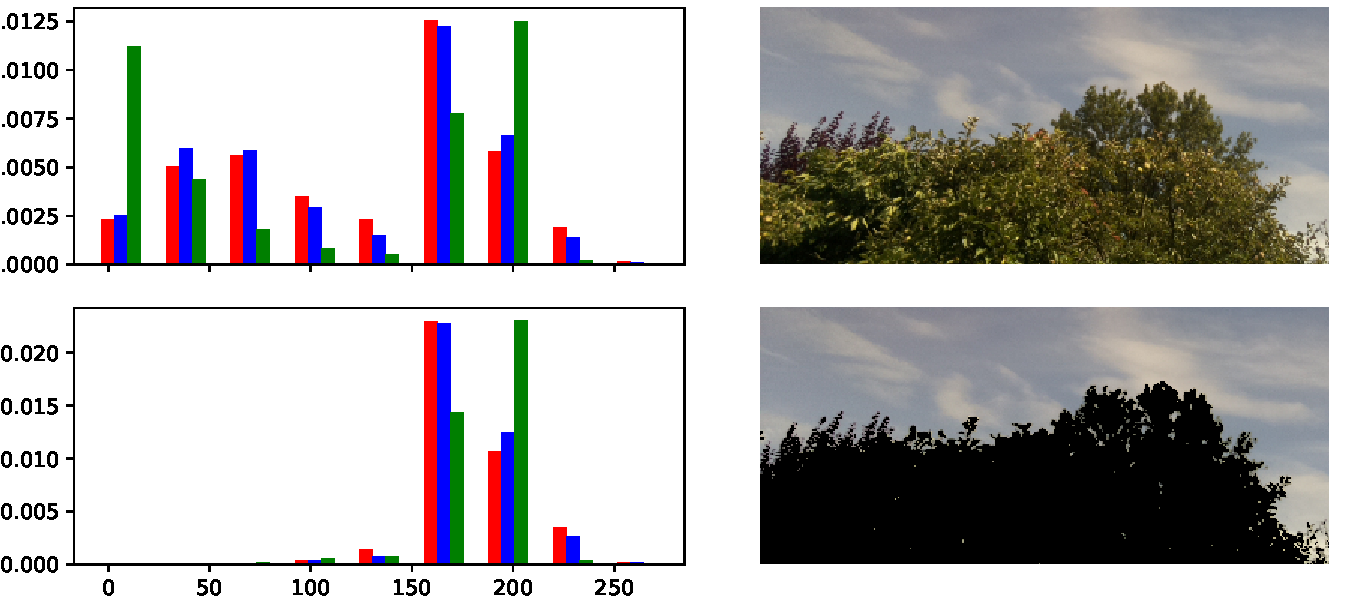
\includegraphics[width=0.8\textwidth]{pictures/cut_hist.pdf}
\caption{Histogramm und Originalfoto mit und ohne Farbschnitt, dargestellt sind nur 10 Bins.}%
\label{fig:cut_hist}
\end{figure}

Der Farbwert $0$ wird nicht in das Histogramm aufgenommen, da sonst
die durch die Farbschnitte entfernten Objekte in die Trainingsdaten
aufgenommen werden würden.

Im letzten Schritt der Vorverarbeitung wird der Datensatz aufgeteilt in
Trainings- und Testdatensatz, die separat in Unterordner gespeichert und
dort in die jeweiligen aufgeteilt Klassen werden. Dies ist notwendig,
damit im Training des Neuronalen Netzes die Funktion
\texttt{flow\_from\_directory} verwendet werden kann, die Batch-weise
Fotos aus den Ordnern lädt, um den Arbeitsspeicher nicht zu überlasten.

Für das Training werden nur 90 bis 150 Bilder pro Klasse verwendet.
Das bedeutet, dass die Klassen `cumulonimbus' und `stratus' nicht klassifiziert werden können.
Die Ausgeglichenheit des Datensatzes ermöglicht jedoch ein von der relativen Häufigkeit der
Klassen unabhängiges Training.

\hypertarget{neuronales-netz}{%
\subsection{Neuronales Netz}\label{neuronales-netz}}

Ein Neuronales Netz wird verwendet, da es in der Lage ist, mittels
\texttt{Convolutional} Schichten Formen auf Bildern zu erkennen. Die
Auswertung besteht aus Matrixmultiplikationen, die einfach zu rechnen sind.
Das Neuronale Netz wird mit dem Python Paket \emph{keras}\footnote{keras.io}
implementiert. Es wird die Klasse \texttt{keras.models.Sequential}
verwendet.

Die Eingangsparameter des Neuronalen Netzes sind die vollständigen
Fotos, also 1024$\times$768$\times$3 Parameter. Die erste Schicht ist eine
\texttt{AveragePooling2D} Schicht, die dazu dient, die Dimension schnell
zu reduzieren. Es werden 3 Abfolgen von \texttt{Convolutional} Schichten
und \texttt{MaxPooling} Schichten verwendet. Die Schichten werden zur
Dimensionsreduktion verwendet. Zusätzlich dazu ist die
\texttt{Convolutional} Schicht geeignet, mittels Faltung Kanten zu
finden und somit fähig, die Form der Wolken zu lernen. Im Anschluss
folgt eine \texttt{Flatten} Schicht, die die
$(n \times N)$-Dimensionalität auf eine
$(n \cdot N \times 1)$-Dimension reduziert. Dies ist notwendig, um im
Anschluss klassische \texttt{Dense} Schichten zu verwenden.

Es folgen \texttt{Dense} Schichten mit 32, 32 und 9 Neuronen, jeweils
gepaart mit \texttt{GaussianNoise} Schichten und \texttt{Dropout}
Schichten, zur Regularisierung. Die \texttt{Dropout} Schichten werden
genutzt, um die Gewichte in einer Größenordnung zu halten, die
\texttt{GaussianNoise} Schichten, um die Gewichte klein zu halten.
Beides ist in der Matrixmultiplikation von Vorteil, da so die genaue
numerische Darstellung von Fließkommazahlen im Rechner möglich ist.

Die Aktivierungsfunktionen sind \texttt{ReLU} in den \texttt{Dense}
Schichten und \texttt{Sigmoid} in der Output-Schicht, um die Vorhersagen
zu normieren. Als Lossfunktion wird \texttt{logcosh} verwendet, da
dieser fehlerhafte Vorhersagen linear bestraft.

\hypertarget{random-forest}{%
\subsection{Random Forest}\label{random-forest}}

Ein Random Forest wird verwendet, da er mit geringem Trainingsaufwand
sehr brauchbare Ergebnisse erzielt. Das Modell ist klein und leicht
rechenbar. Der Random Forest wird mit dem Python Paket
\emph{scikit-learn}\footnote{scikit-learn.org} implementiert. Es wird
die Klasse \linebreak\texttt{sklearn.ensemble.RandomForestClassifier} verwendet.

Die Eingangsparameter des Random Forest sind die histogrammierten
Farbkanäle der Fotos, auf denen die Farbschnitte angewendet wurden. Die
Trainingsdaten haben die Dimension $(N \times 90)$.

Der einzige wichtige Hyperparameter ist hier \texttt{n\_estimators}. Er
entscheidet, wie viele Bäume im Random Forest verwendet werden. Es wird
$\texttt{n\_estimators} = 300$ gewählt, da durch eine hohe Anzahl an
Bäumen Overfitting verhindert wird.

\hypertarget{darstellung-und-interpretation-der-ergebnisse}{%
\section{Darstellung und Interpretation der
Ergebnisse}\label{darstellung-und-interpretation-der-ergebnisse}}

Die nachfolgend dargestellten Untersuchungen des Datensatzes werden mit
Random Forest durchgeführt, da dieser um Größenordnungen schneller
trainiert.

\hypertarget{nichtuxfcbereinstimmung-der-label-auf-dem-datensatz}{%
\subsection{Nichtübereinstimmung der Label auf dem
Datensatz}\label{nichtuxfcbereinstimmung-der-label-auf-dem-datensatz}}

Bei der Einteilung des Datensatzes in die Unterordner der jeweiligen
Klassen des Trainings- und Testdatensatzes ist aufgefallen, dass die
zugeordneten Label teilweise nicht mit den Klassen übereingestimmt
haben. Bei der Inspektion des Codes für das Labeln ist klar geworden,
dass sich parallele Threads beim Labeln mehrerer Personen gleichzeitig
überschrieben haben und somit falsche Label zu den Fotos zugeordnet
worden sind.

Um die falsch gelabelten Fotos zu korrigieren, wird ein simpler Random
Forest auf einem kleinen Teil des fehlerhaften Datensatz trainiert und
auf dem gesamten Datensatz ausgewertet. Bei Klassifizierungen, die nicht
mit dem von uns gesetzten Label übereinstimmten, haben wir mit einer
binären Entscheidung (\enquote{stimmt} / \enquote{stimmt nicht}) das von uns
gesetzte Label bestätigt oder verworfen. Dazu wurde der Code zum Labeln
und der Telegram-Bot erweitert. Die verworfenen Fotos mussten neu
gelabelt werden.

Dieser Vorgang wurde mehrere Male wiederholt, bis ein fehlerfrei
gelabelter Datensatz entstand.

Ein Random Forest ist zusätzlich zu den oben genannten Argumenten für
diese Aufgabe geeignet, da dieser robuster als ein Neuronales Netz gegen
falsche Label im Training ist.

Im Anschluss können sowohl ein finaler und auf reinem Datensatz
trainierter Random Forest sowie ein Neuornales Netz trainiert werden.

\hypertarget{neuronales-netz-1}{%
\subsection{Neuronales Netz}\label{neuronales-netz-1}}

Das Neuronale Netz wird 200 Epochen trainiert. Als Metrik wird
\texttt{categorial\_accuracy} verwendet. Dies ist die Genauigkeit bei
der Klassifizierung einer einzelnen Klasse, gemittelt über alle Klassen.

Die Genauigkeit und der Loss werden auf den Trainings- und Testdaten
gegen die Epoche in Abbildung~\ref{fig:train_nn} dargestellt. Es ist zu erkennen, dass die
Werte in Sättigungswerte laufen, die für den Validierungsdatensatz (gepunktete Linie) bei
\begin{align}
  ACC  &=  \num{0.65} \\
  LOSS &= \num{0.35}
\end{align}
liegen.

\begin{figure}
\centering
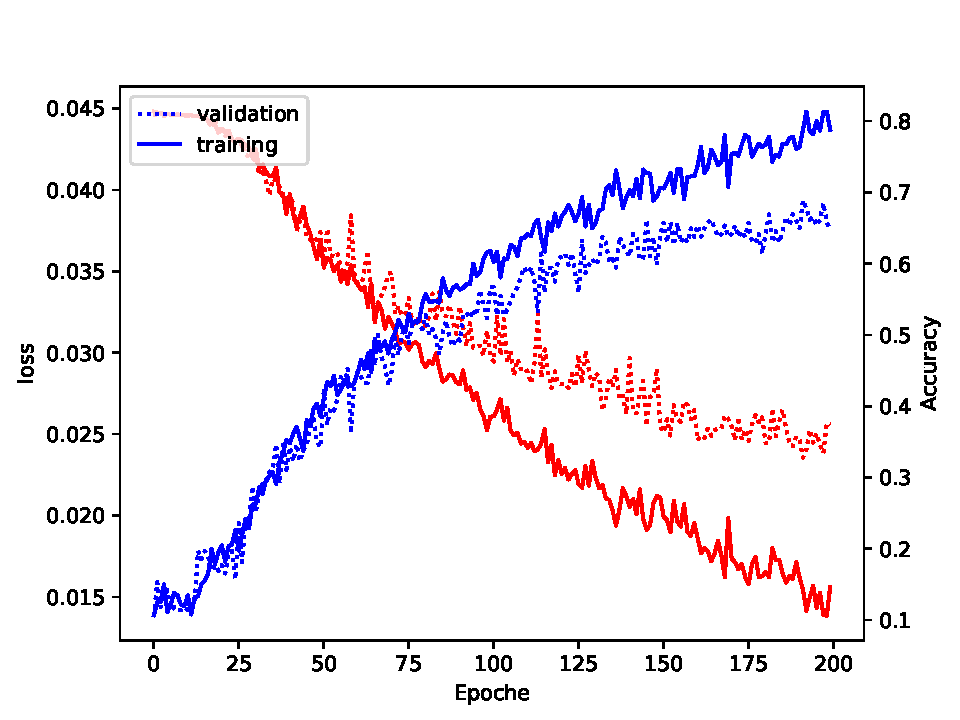
\includegraphics[width=0.8\textwidth]{content/train_nn.pdf}
\caption{Trainings- und Validierungsloss und -genauigkeit.}%
\label{fig:train_nn}
\end{figure}

Die Confusion Matrix in Abbildung~\ref{fig:conf_nn} zeigt, welche Klassen besser und
welche schlechter vorhergesagt werden.
Insbesondere die Klasse `cumulus' wird mit 95\% Genauigkeit vorhergesagt.
Dies liegt an der deutlich ausgeprägten Form und und den harten Unterschieden in den Farben.
Ein Beispiel für eine Cumuluswolke ist im Anhang in Abbildung~\ref{fig:cumulus} zu finden.
Die Klasse `cirrus' wird schlecht vorhergesagt.
Gründe hierfür sind geringe Farbunterschiede und diffuse Formen.
Ein Beispiel für eine Cirruswolke ist im Anhang in Abbildung~\ref{fig:cirrus} zu finden.


\hypertarget{random-forest-1}{%
\subsection{Random Forest}\label{random-forest-1}}

Der finale Random Forest, der die Alternativmethode zum Neuronalen Netz
darstellt, erreicht eine Genauigkeit auf dem Testdatensatz von 74\%.
An der Confusion Matrix in Abbildung~\ref{fig:conf_rf} ist eindeutig zu erkennen, welche
Wolkenklassen gut, und welche schlecht voneinander getrennt werden
können.

Eindeutig zu erkennen ist, dass die Klassen `nimbostratus' und `no clouds' gut
vom Random Forest vorhergesagt werden kann, während die Klassen
`cirrus' und `cirrocumulus' schlecht klassifiziert werden
können.
Dies liegt im ersten Beispiel an der hohen Homogenität der Farbe über das gesamte Foto.
Dass insbesondere `cirrus' als `no clouds' klassifiziert wird,
liegt an der diffusen Form der Cirruswolke und den deswegen geringen Farbunterschieden der beiden
Fotos.
Siehe auch hier Abbildung~\ref{fig:cirrus}.

Die Auswertungszeiten der Modelle sind in Abbildung~\ref{fig:times} dargestellt.
Falls diese nicht mit den Zeiten im Code übereinstimmen, liegt dies an der Auswahl an
Fotos, da nicht der gesamte Datensatz abgegeben wird.

\begin{figure}
  \centering
  \begin{subfigure}[t]{0.48\textwidth}
    \centering
    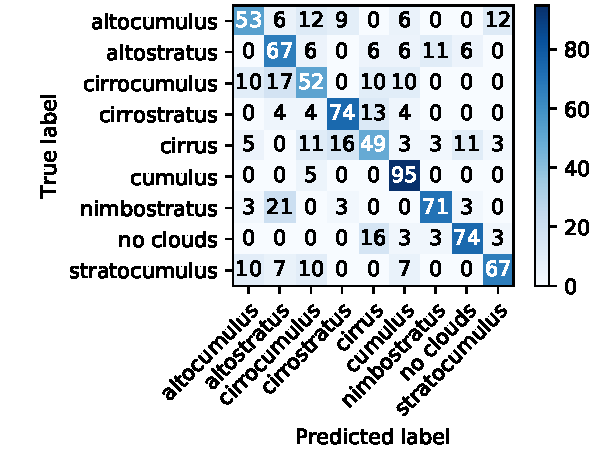
\includegraphics[width=\textwidth]{content/conf_nn.pdf}
    \caption{Confusion Matrix für das Neuronale Netz.}%
    \label{fig:conf_nn}
  \end{subfigure}
  \begin{subfigure}[t]{0.48\textwidth}
    \centering
    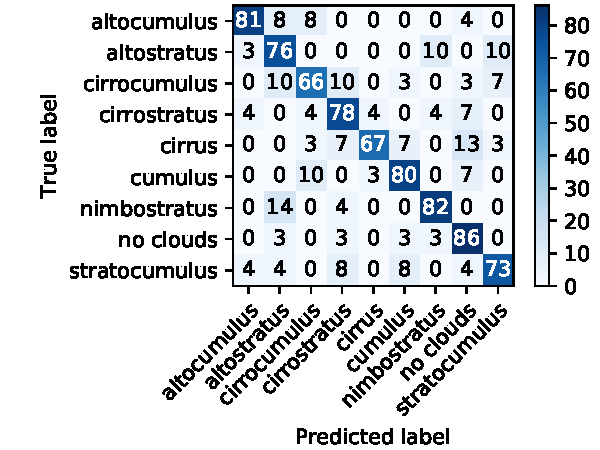
\includegraphics[width=\textwidth]{content/conf_rf.pdf}
    \caption{Confusion Matrix für den Random Forest.}%
    \label{fig:conf_rf}
  \end{subfigure}
  \caption{Confusion Matrizen der Modelle.}%
  \label{fig:conf_mat}
\end{figure}


\begin{figure}
\centering
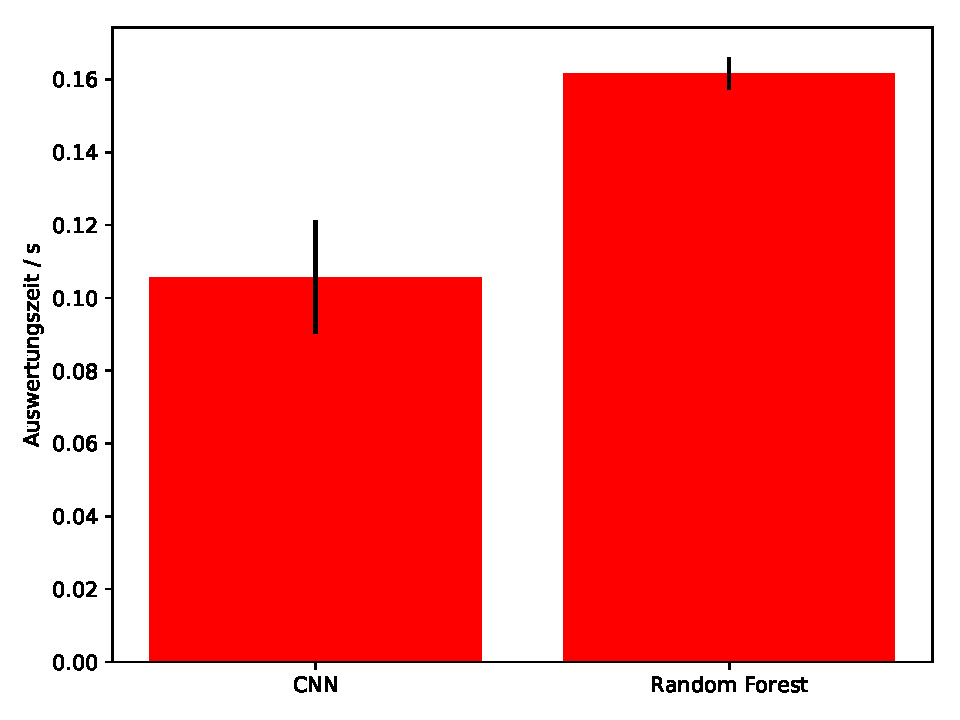
\includegraphics[width=0.7\textwidth]{content/time.pdf}
\caption{Vergleich der Auswertungszeiten von Neuronalem Netz und Random
Forest.}%
\label{fig:times}
\end{figure}

\hypertarget{zusammenfassung}{%
\section{Zusammenfassung}\label{zusammenfassung}}

Ein erstes Ergebnis dieser Arbeit ist die Bestätigung, dass ein Random
Forest robust gegen falsche Label im Datensatz ist. Dies liegt an der
Mittelung über viele Entscheidungsbäume.

Der Random Forest erreicht eine höhere Leistung, als das Neuronale Netz,
bezogen auf die Problemstellung.

\begin{table}
  \centering
  \caption{Vergleich der relevanten Metriken.}%
  \label{tab:fazit}
  \begin{tabular}[]{@{}lrr@{}}
    \toprule
    Merkmal             & Neuronales Netz & Random Forest \\
    \midrule
    Genauigkeit / \%    & 64              & 74            \\
    Auswertungszeit / s & 0.11            & 0.16          \\
    \bottomrule
  \end{tabular}
\end{table}

Jedoch ist das Neuronale Netz in der Auswertung schneller, als der
Random Forest (s.~Tabelle~\ref{tab:fazit}).

Es muss berücksichtigt werden, dass der Random Forest einen
Trainingsdatensatz einer viel geringeren Dimension hat.

Aus diesen Gründen ist die Alternativmethode für die
Wolkenklassifikation besser geeignet, als die gewählte Methode des
maschinellen Lernens.

Es hat sich herausgestellt, dass die Problemstellung mit einem recht
simplen Algorithmus besser beantwortet werden kann, als mit einem
komplizierteren. Dies ist jedoch nur möglich, da die
Vorverarbeitungsschritte gut überlegt und implementiert sind. Der
Vorteil der Implementierung der Vorverarbeitung ist, dass jedes mögliche
Foto gefiltert werden kann, und sie nicht auf die Bildgröße 1024$\times$768
beschränkt ist. Außerdem kann ein anderer Farbraum geschnitten werden,
wenn eine gute Schnittfunktion gefunden wurde.

Die durchschnittliche Genauigkeit von 74\% bei einer Klassifikation in 9 Klassen
ist ein sehr guter Wert.
An der Confusion Matrix wird deutlich, welche Klassen besser und welche schlechter vorhergesagt
werden können.
Diese Klassen unterscheiden sich in den Daten sehr gering,
sodass zusätzliche Vorverarbeitungscchritte sinnvoll sind.
Ein mehrstufiges System,
das zum Beispiel erst Wolken von `no clouds' trennt
und im Anschluss die Cirrus-Wolkentypen einzeln klassifiziert,
kann hier von Vorteil sein.

\newpage

\hypertarget{anhang}{%
\section*{Anhang}\label{anhang}}
\addcontentsline{toc}{section}{Anhang}

Um den Code auszuführen, sollte eine virtuelle Umgebung für Python
verwendet werden. Mit iner aktuellen Installation von \texttt{conda} ist
die möglich. Im Ordner \texttt{weatherpi} wird
\texttt{pip\ install\ -e\ .} und
\texttt{pip\ install\ -r\ requirements.txt} (in der Reihenfolge)
gerufen, um die notwendigen Pakete zu installieren. Im Ordner
\texttt{weatherpi/predictions/pipeline/} wird mit
\texttt{python\ pipeline.py} die gesamte Analyse durchgeführt. Die Daten
liegen in \texttt{weatherpi/predicitons/pipeline/data} und die Label in
der Datei \linebreak\texttt{weatherpi/predictions/pipeline/label.pkl}.

Im Folgenden sind die Kommandos erneut aufgelistet, auszuführen im Order
\texttt{weatherpi}.

\begin{verbatim}
conda create -n bdrbcksckl python=3.6 pip
conda activate bdrbcksckl
pip install -e .
pip install -r requirements.txt
cd predictions/pipeline
python pipeline.py
\end{verbatim}

\newpage

\begin{figure}[ht]
  \centering
  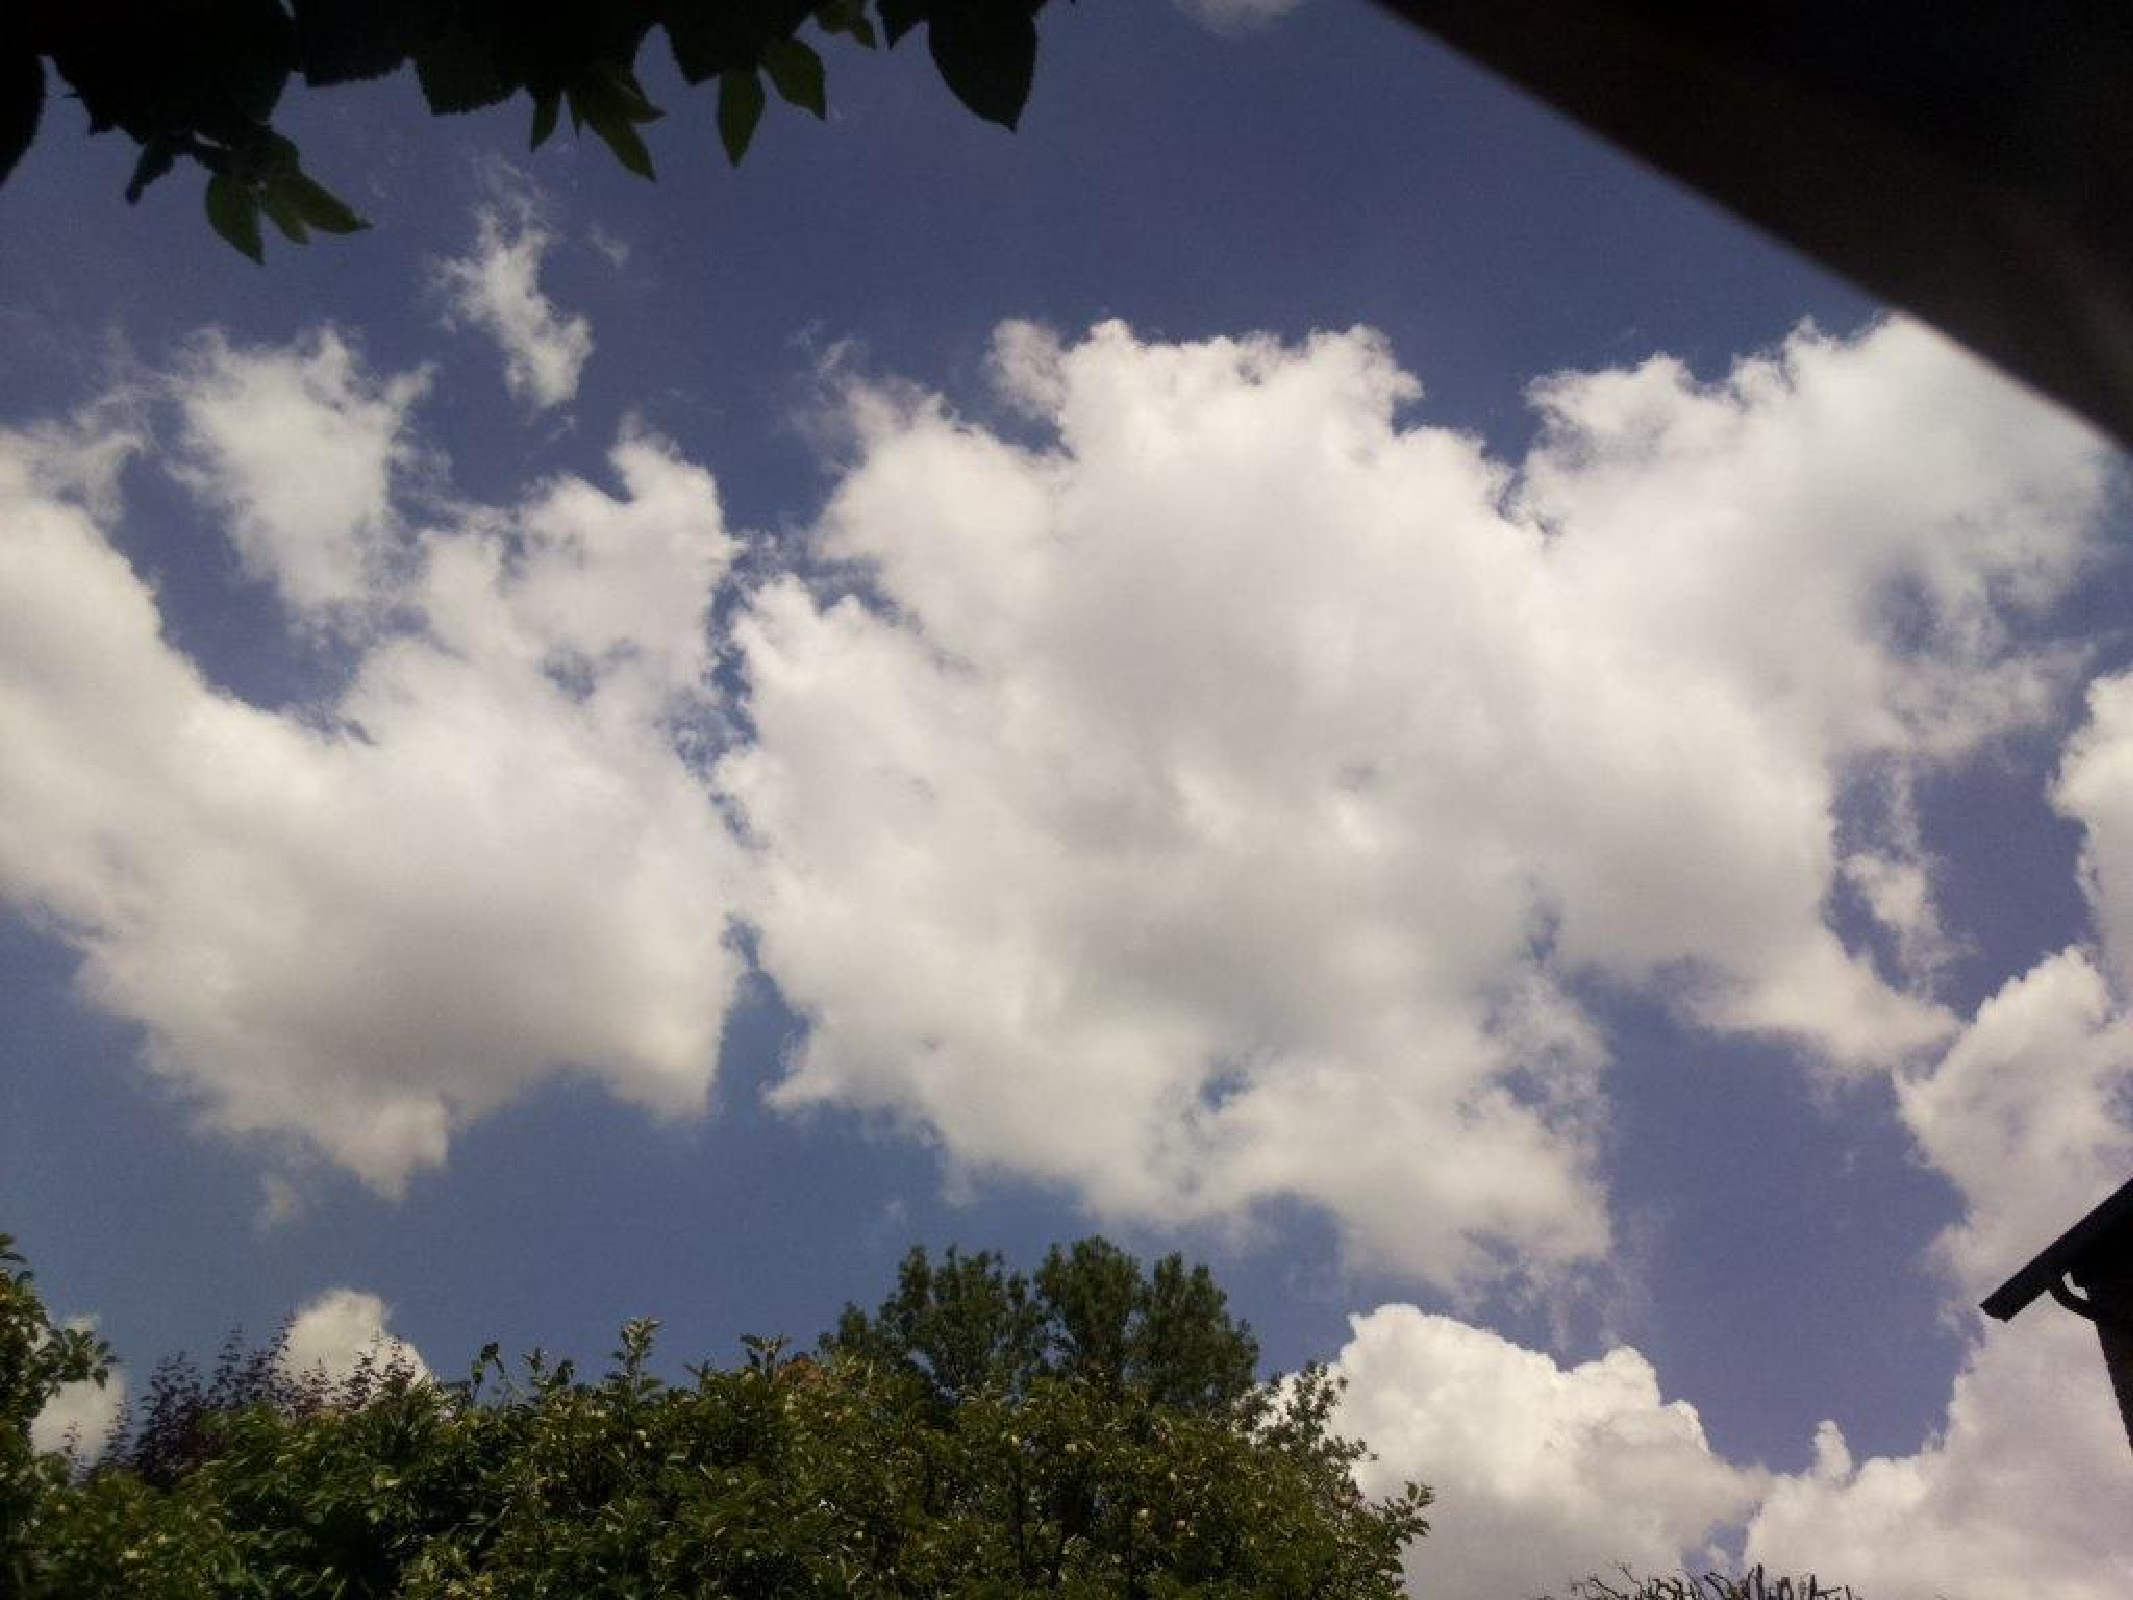
\includegraphics[height=0.25\textheight]{content/cumulus.pdf}
  \caption{Beispiel für eine Cumuluswolke. Gut zu erkennen sind Form und Farbunterschiede. Dies
  sind die Gründe für die gute Klassifikation des Neuronalen Netzes.}
  \label{fig:cumulus}
\end{figure}

\begin{figure}[ht]
  \centering
  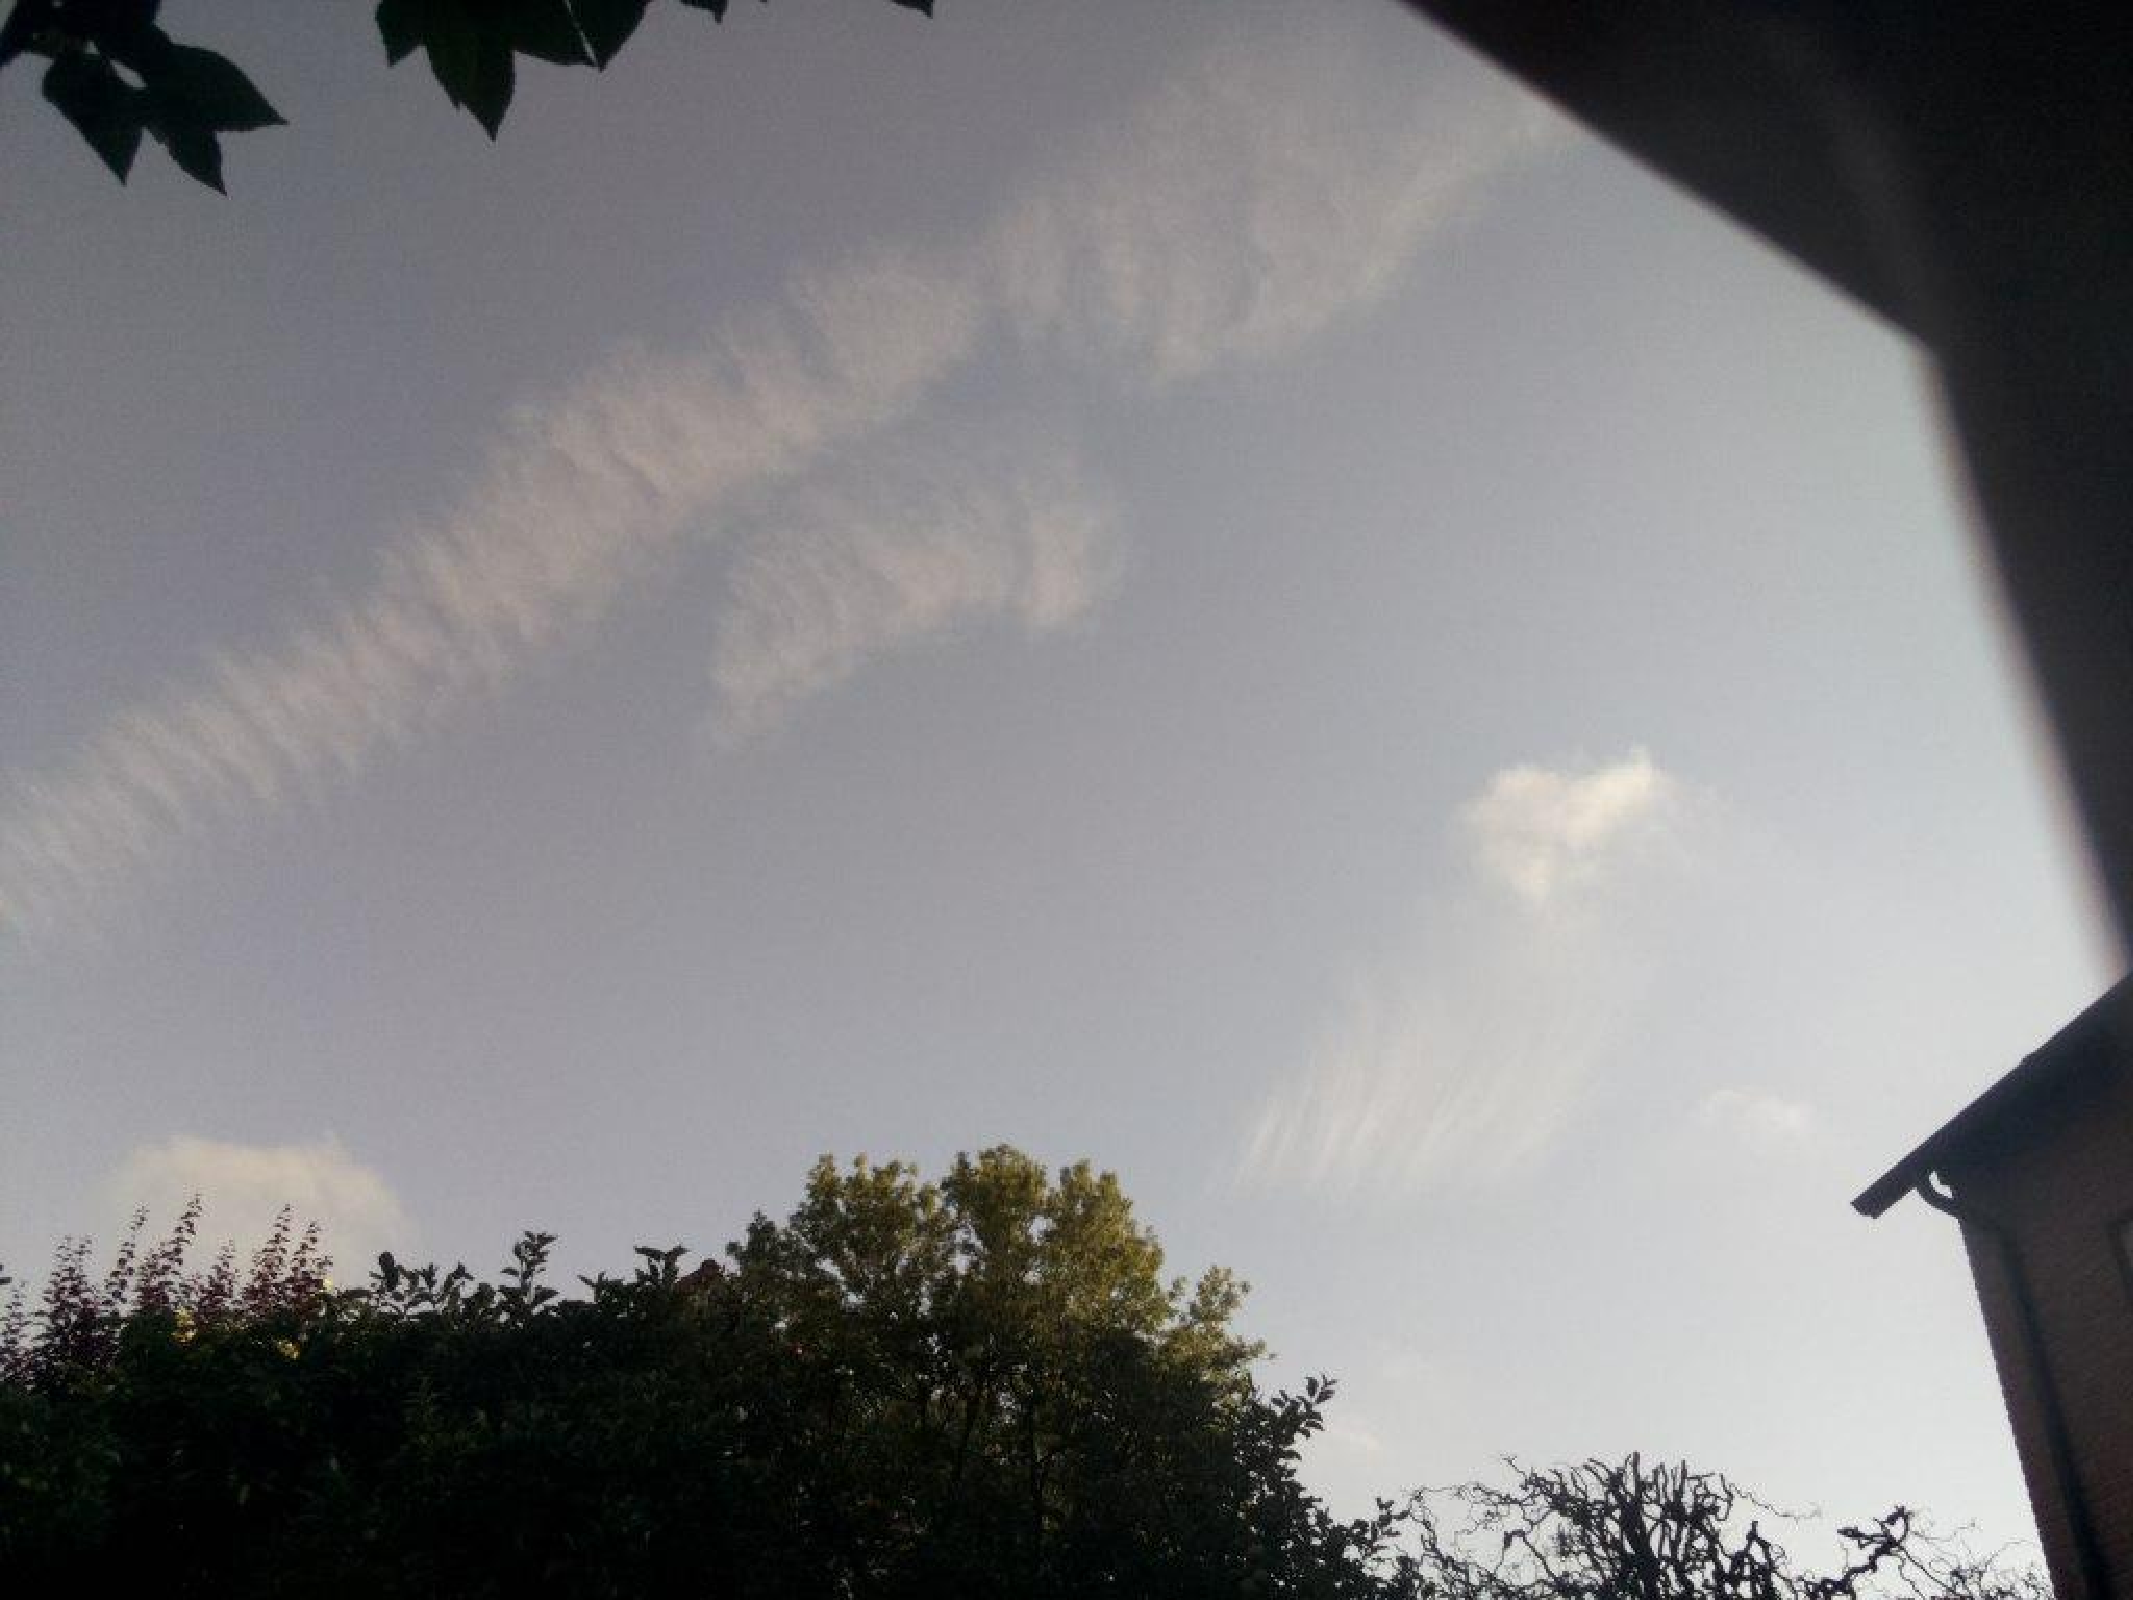
\includegraphics[height=0.25\textheight]{content/cirrus.pdf}
  \caption{Beispiel für eine Cirruswolke. Gut zu erkennen sind die diffuse Form und geringe Farbunterschiede. Dies
  sind die Gründe für die schlechte Klassifikation des Neuronalen Netzes.}
  \label{fig:cirrus}
\end{figure}
